\chapter{Neuronové sítě}
\label{sec:NN}

Umělá neuronová síť (ang. Artificial Neural Network - ANN) nebo jen neuronová
síť (ang. Neural Network - NN) je výpočetní model inspirovaný biologickými
nervovými systémy v lidském mozku. Na rozdíl od konvenčních výpočetních modelů,
které zpracovávají informace algoritmicky, a tedy postupují dle předem určeného
postupu, se informace v tomto modelu šíří v síti váh mezi jednotlivými neurony.
Jelikož je výstup ze sítě dané architektury závislý hlavně na numerických
parametrech, zejména váhách jednotlivých spojů mezi neurony, lze funkčnost sítě
měnit bez změny programu pouhou změnou těchto parametrů, a to i automaticky v
procesu trénování modelu.

Nyní krátce projdeme historií vývoje neuronových s síti.

\section{Historie}
\label{sec:NN_History}

\subsection{Prvopočátky}
První matematický model neuronové sítě byl popsán v roce 1943 dvěma
neurofyziology - Warrenem McCullochem a Walterem Pittsem. \cite{McCulloch1943}
Model byl založen na síti jednoduchých logických prvků, které provedou vážený
součet svých vstupů a na výstup odešle signál založený na prahové funkcí.

V roce 1958 pak Frank Rosenblatt představil elektronicky model neuronové sítě.
Základní jednotku, postavenou na McCulloch-Pittsově modelu, nazval perceptron.
\cite{Rosenblatt1958} Jeho architektura byla podobná modelu znázorněnému na
obrázku \ref{fig:neuron}, kde aktivační funkce je prahová funkce. Rosenblattův
stroj - Mark I Perceptron - byl postavený pro rozpoznávání jednoduchých vzorů v
obrazech. Hlavním omezením tohoto modelu bylo, že byl schopen rozlišovat pouze
lineárně separovatelné třídy.

Další systém - ADALINE (Adaptive Linear Neuron) - byl představen Bernardem
Widrowem and Tedym Hoffem v roce 1960. Tento model umělého neuronu byl velmi
podobný perceptronu, na rozdíl od něj ale neobsahoval prahovou ale lineární
funkcí, výstup tedy nebyl binární ale spojitý. Pro učení pak byla využitá
metoda nejmenších čtverců, která minimalizovala chybu mezi skutečným a
očekávaným výstupem. \cite{nn_history}

I když ve svých počátcích přitahoval koncept umělé inteligence mnoho vědců jako
i sponzorů, v následujících létech zájem ochabl, jelikož nebylo dosaženo
předpokládaných výsledků, hlavně s ohledem na tehdejší stav vývoje hardwaru a
obecně výpočetní techniky. Proto se tomuto období někdy říká Ai Winter.
Neznamená to ale, že ti, kteří se oboru nadále věnovali, nedosáhli významných
výsledků. \cite{nn_history}

\subsection{Objev backpropagation}
Významným milníkem v historii neuronových sítí byl objev algoritmu
backpropagation, zvaného taky algoritmus zpětného šíření chyby. Tento
algoritmus byl vyvinut v roce 1974 Paulem Werbosem, popularitu ale dosáhl až po
nezávislém objevení v roce 1986 Davidem Rumelhartem et al.
\cite{backpropagation}

Tento algoritmus umožnil trénovat sítě s více vrstvami, což položilo základ
hlubokému učení. Algoritmus využívá metodu gradientního sestupu v kombinaci s
řetězovým pravidlem derivací k nalezení optimálních vah sítě vedoucích k
minimalizaci chyby.

Vynález backpropagation byl jedním z hlavních důvodů, proč se v 80. letech
obnovil zájem o neuronové sítě a umělou inteligenci obecně. 



\begin{figure}[]
    \centering
    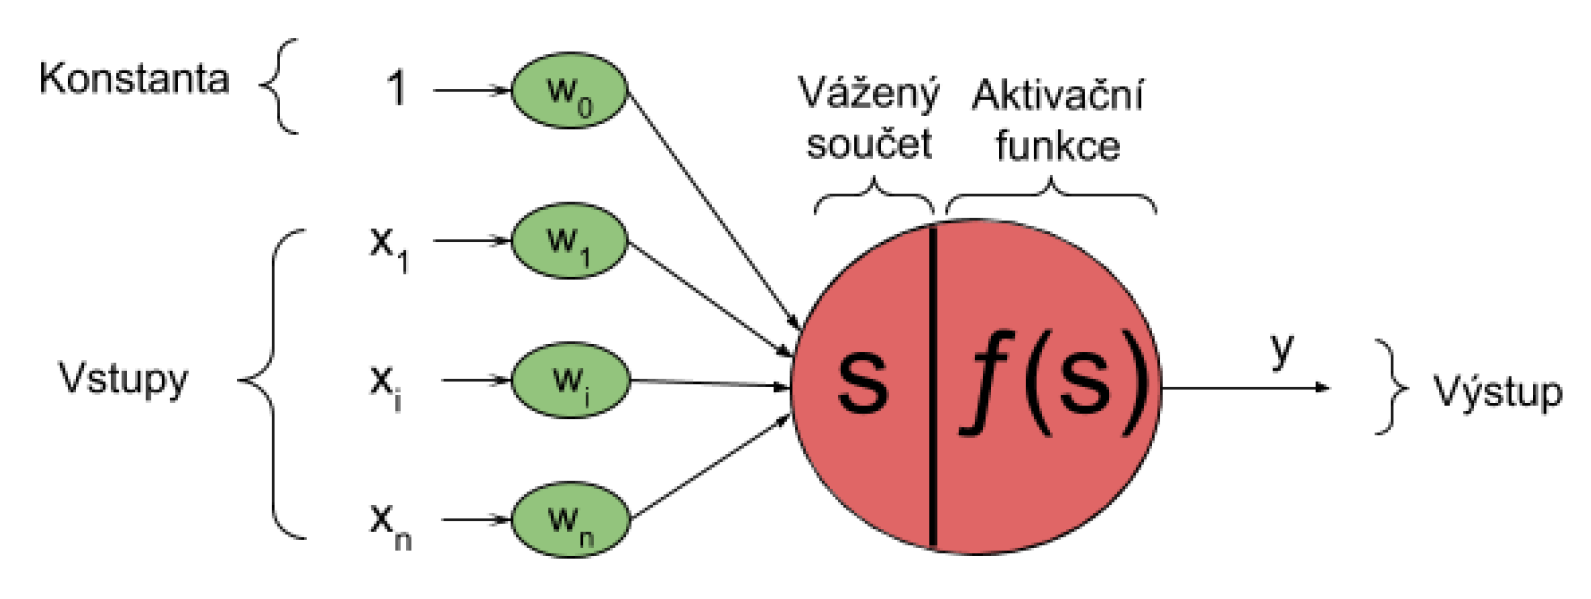
\includegraphics[width=0.5\textwidth]{Figures/neuron.png}
    \caption{Model umělého neuronu \cite{lagan}}
    \label{fig:neuron}
\end{figure}

\endinput